\documentclass[12pt,a4paper]{article}
\usepackage[margin=1in]{geometry}
\usepackage{amsmath,amssymb,graphicx,booktabs,hyperref,fancyhdr}
\setlength{\headheight}{15pt}
\pagestyle{fancy}
\fancyhf{}
\lhead{Problem A -- UPC 2026}
\rhead{Team: 758}
\cfoot{\thepage}
\newcommand{\draftnote}[1]{\par\noindent\textit{Draft plan: #1}\par}
\title{P1: Dynamics Derivation and Internal Verification}
\author{Problem A \qquad Team Control Number: 758}
\date{}

\makeatletter
\setlength{\@fptop}{0pt}
\makeatother
\begin{document}
\maketitle
\noindent This P1 report establishes and verifies the reference dynamics. Whole-flight guidance and fuel optimization are outside its scope.
\setcounter{section}{3}
\section{Model Force Analysis}
\subsection{Gravity and Standard Atmosphere}
We use a local downrange--vertical plane. Position refers to the center of mass (COM), and the pitch angle points from the tail toward the nose. Gravity acts through the COM and has magnitude
\begin{equation}
 g(h)=g_0\left(\frac{R_E}{R_E+h}\right)^2,\qquad g_0=9.80665\ \mathrm{m/s^2},\quad R_E=6356766\ \mathrm m.
\end{equation}
At 70 km this gives $g=9.5942\ \mathrm{m/s^2}$, about 2.17\% below $g_0$. This is a spherical, nonrotating reference approximation, not a latitude-resolved gravity model.

Atmospheric properties follow the lower layers of the 1976 standard atmosphere~\cite{atmosphere}. Geometric altitude $h$ is converted to geopotential altitude $H=R_Eh/(R_E+h)$. In a layer with base $(H_b,T_b,p_b)$ and temperature gradient $\lambda$,
\begin{align}
 T_a&=T_b+\lambda(H-H_b),\\
 p_a&=\begin{cases}p_b(T_a/T_b)^{-g_0/(R_a\lambda)},&\lambda\ne0,\\p_b\exp[-g_0(H-H_b)/(R_aT_b)],&\lambda=0,\end{cases}\\
 \rho&=\frac{p_a}{R_aT_a},\qquad R_a=287.05287\ \mathrm{J/(kg\,K)}.
\end{align}
These expressions follow from hydrostatic balance $dp_a/dH=-\rho g_0$ and the ideal-gas law. The implemented range ends at $H=84.852$ km; trajectories outside that range are rejected rather than assigned extrapolated density.

\subsection{Axial and Crossflow Aerodynamics}
The cylindrical approximation gives $A_{end}=\pi D^2/4=38.4845\ \mathrm{m^2}$ and side area $DL=455\ \mathrm{m^2}$. Define body directions
\begin{equation}
 \mathbf e=(\cos\theta,\sin\theta),\quad \mathbf n=(-\sin\theta,\cos\theta),\quad
 \mathbf u=\mathbf v-\mathbf w,\quad u_a=\mathbf u\cdot\mathbf e,\quad u_n=\mathbf u\cdot\mathbf n.
\end{equation}
Instead of applying one coefficient to a changing projected area, we separate axial and crossflow contributions. Cylinder research motivates treating crossflow as a distinct aerodynamic regime~\cite{cylinder}; our constant coefficients are low-order engineering assumptions, not a fit to that report.

The axial force is
\begin{equation}
 F_a=-\tfrac12\rho C_a A_{end}u_a|u_a|.
\end{equation}
For an equivalent crossflow strip at signed axial arm $s$, rotation adds the local normal velocity $\omega s$. Thus
\begin{equation}
 dF_n=-\tfrac12\rho C_nD(u_n+\omega s)|u_n+\omega s|\,ds.
\end{equation}
With $N$ midpoint strips of length $\Delta s=L/N$ and $s_i=-L/2+(i-1/2)\Delta s+\Delta l$,
\begin{equation}\label{eq:strip}
 \mathbf F_D=F_a\mathbf e+\sum_iF_{n,i}\mathbf n,\qquad M_a=\sum_i s_i F_{n,i}.
\end{equation}
The shifted equivalent distribution represents an uncertain pressure-center offset $\Delta l$; it is not a physical surface mesh. We evaluate density at the COM and neglect its variation across the 65 m body. Axial force acts along the centerline. Figure~\ref{fig:forces} defines the forces and signs.

For zero rotation, $M_a=\Delta l F_n$. Consequently, even spatially uniform wind can generate a moment when $\Delta l\ne0$. For a centered distribution and pure rotation, direct integration gives
\begin{equation}\label{eq:rotation}
 M_a=-\frac{\rho C_nD L^4}{64}\omega|\omega|.
\end{equation}
This opposes rotation. More generally, the mechanical power transferred by the modeled air-relative forces satisfies
\begin{equation}
 \mathbf F_D\cdot\mathbf u+M_a\omega
 =-\tfrac12\rho C_aA_{end}|u_a|^3-\tfrac12\rho C_nD\sum_i\Delta s|u_n+\omega s_i|^3\le0.
\end{equation}
This identity provides a useful sign and implementation check. It concerns motion relative to air, not ground-frame energy in moving wind.
\begin{figure}[htbp]\centering
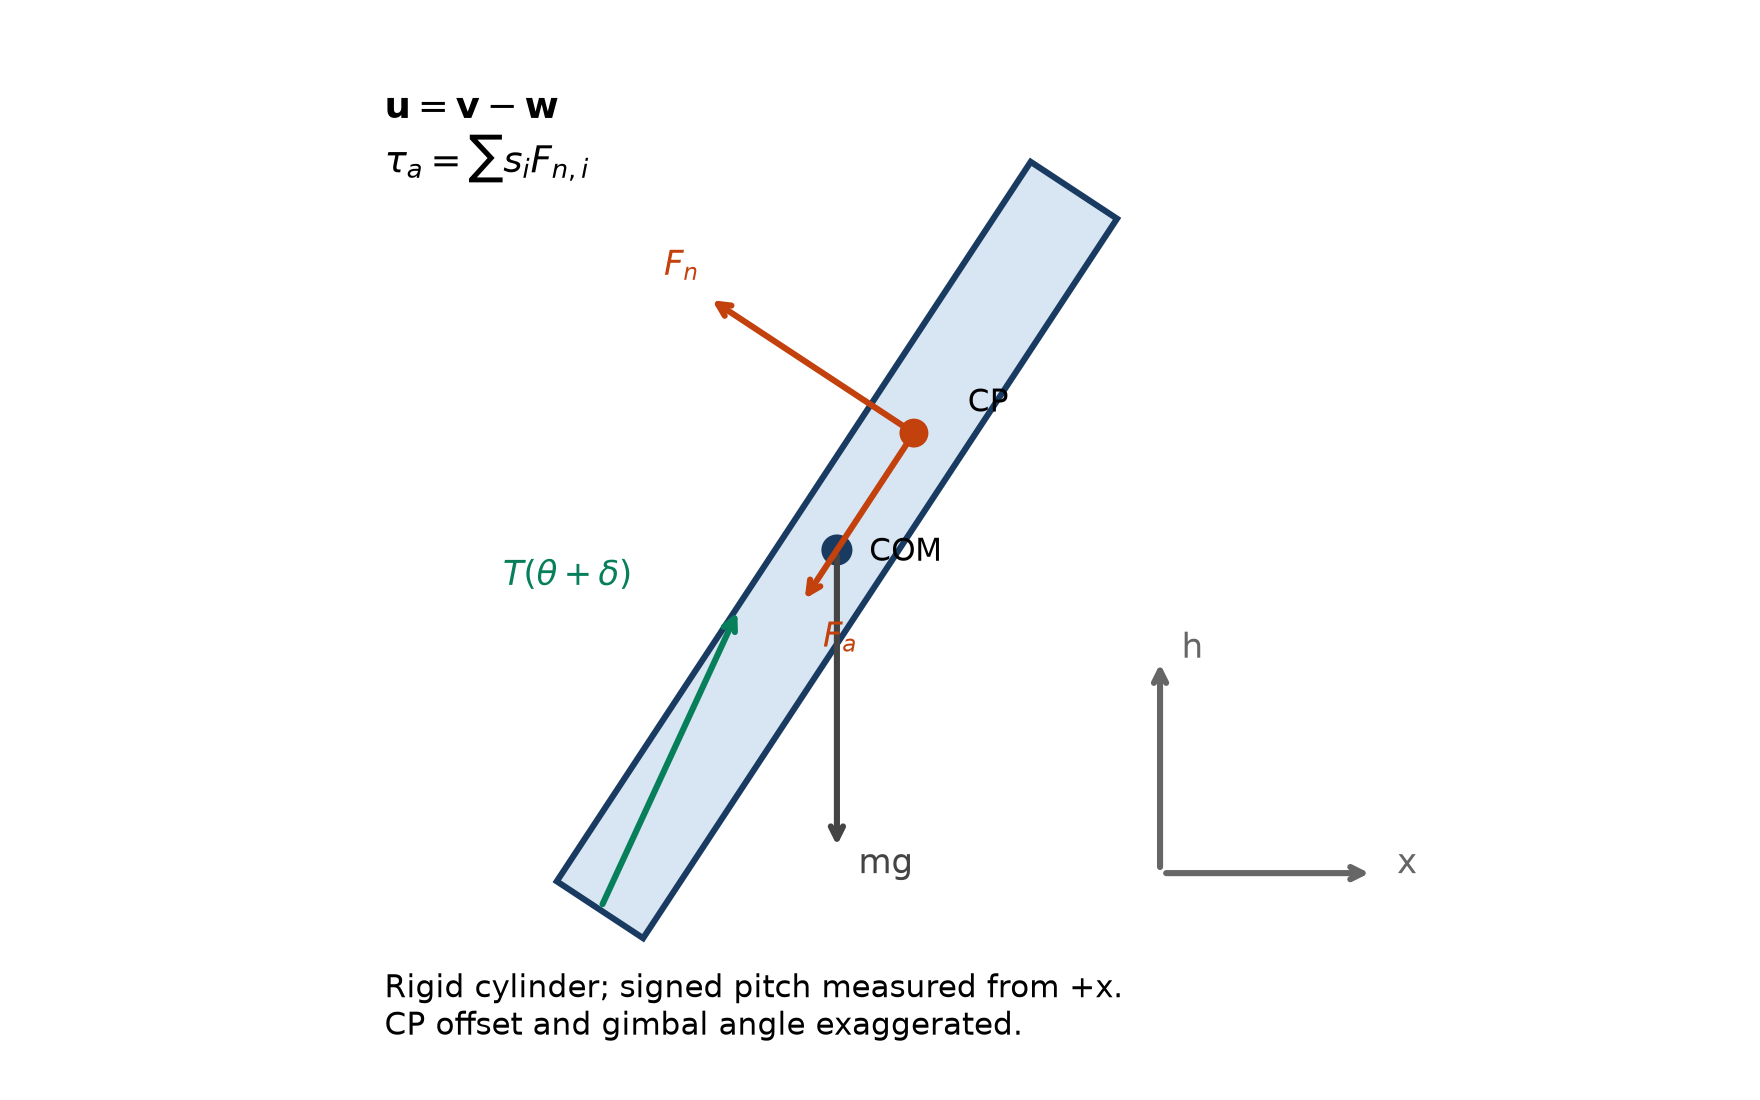
\includegraphics[width=.88\linewidth]{figure/p1-forces.png}
\caption{Planar reference geometry and force conventions. The pressure-center displacement is exaggerated. Positive gimbal angle at the tail produces a negative pitch moment.}\label{fig:forces}
\end{figure}

\subsection{Reference Propulsion Parameters}
The maximum landing thrust is set to 2.846 MN by analogy with the published BE-4 thrust scale~\cite{be4}. We select effective $I_{sp}=330$ s, oxygen-to-methane mass ratio 3.5, minimum throttle 0.4, and gimbal limit $10^\circ$ as reference-design assumptions. The mixture-ratio choice is informed by a methane/oxygen mission study~\cite{methaneStudy}; that study's vacuum specific impulse is not assigned to this landing engine. We set $C_a=0.8$, $C_n=1.2$, and $\Delta l=0.05L$. The P0 reference contract records exploratory scenario points. We report selected efficiency and crossflow comparisons and retain explicit limitations for unexamined assumptions.

The standard effective-exhaust-velocity definition gives $c=I_{sp}g_0$ and
\begin{equation}
 \dot m=-T/c,\qquad T=0\quad\hbox{or}\quad0.4T_{max}\le T\le T_{max}.
\end{equation}
This consumes both oxygen and methane. Pressure dependence and actuator transients are represented only through the effective parameter assumptions at this stage.

\section{Model Motion Analysis}
\subsection{Momentum Balance and Pitch Dynamics}
The state is $\mathbf y=(x,h,v_x,v_h,m,\theta,\omega)$. Accounting for exhaust momentum through thrust, the open-system translational balance is $m\dot{\mathbf v}=m\mathbf g+\mathbf F_D+\mathbf F_T$. One must not add a second $\dot m\mathbf v$ term to this thrust-based equation. The planar baseline used to initialize the corrected calculation is
\begin{align}\label{eq:dynamics}
 \dot x&=v_x,&\dot h&=v_h,\\
 \dot v_x&=\frac{F_{D,x}+T\cos(\theta+\delta)}m,&
 \dot v_h&=-g(h)+\frac{F_{D,h}+T\sin(\theta+\delta)}m,\\
 \dot m&=-\frac T{g_0I_{sp}},&\dot\theta&=\omega,\\
 I_d\dot\omega&=M_a-\frac L2T\sin\delta,&
 I_d&=\frac{m_d(3R_b^2+L^2)}{12}.
\end{align}
The thrust application point is $-(L/2)\mathbf e$, so its cross product with thrust gives the negative sign above. The dry body is modeled as a uniform cylinder. Remaining propellant is idealized as concentrated at the COM with negligible pitch inertia and no additional rotational angular-momentum flux. Hence $I_d$ is constant. A distributed-tank model would require consistent treatment of changing inertia and exhaust angular momentum; the present equation does not claim to describe those effects.

\subsection{Spherical-Earth Correction}
The adopted correction uses a nonrotating spherical Earth with radius $R_E$. Write $r=R_E+h$ and $s=R_E\phi$, where $s$ is surface arc distance. Velocities $v_x$ and $v_h$ are physical components along the changing local horizontal and radial directions. The state retains the seven-component layout, with $x$ replaced by $s$. Let $a_x=F_x/m$ and $a_h=F_h/m$ denote non-gravitational accelerations. Differentiating the moving basis gives
\begin{align}\label{eq:sphere}
 \dot s&=\frac{R_E}{r}v_x,&\dot h&=v_h,\\
 \dot v_x&=a_x-\frac{v_xv_h}{r},&
 \dot v_h&=a_h-g(h)+\frac{v_x^2}{r}.
\end{align}
Thus surface distance differs from the integral of local horizontal speed, and both acceleration components acquire curvature terms.

We retain $\omega=\dot\theta$ as pitch rate relative to the local horizontal. As that horizontal rotates at $-v_x/r$ in the flight plane, inertial body rate is $\omega_I=\omega-v_x/r$. The strip velocity in Eq.~\eqref{eq:strip} uses $u_n+\omega_I s_i$. The consistent angular equation is
\begin{equation}\label{eq:spherepitch}
 \dot\omega=\frac{M_a+M_T}{I_d}+\frac{a_x}{r}-\frac{2v_xv_h}{r^2}.
\end{equation}
The last two terms are obtained by differentiating $v_x/r$. This distinction preserves torque-free inertial rotation while allowing the local vertical to change along the trajectory.

For sea-level contact, the cylindrical longitudinal section is a rectangle in the local flight plane. The point nearest the Earth center has body coordinates
\begin{equation}
 a_* = \operatorname{clip}(-r\sin\theta,-L/2,L/2),\qquad
 b_* = \operatorname{clip}(-r\cos\theta,-R_b,R_b).
\end{equation}
The event function is
\begin{equation}\label{eq:spherecontact}
 f_s=\sqrt{(a_*\cos\theta-b_*\sin\theta)^2+(r+a_*\sin\theta+b_*\cos\theta)^2}-R_E-h_{deck}.
\end{equation}
It uses the radial surface and the full cylinder section. Ship position is a fixed surface arc coordinate. The 5 m targeting tolerance keeps the local deck orientation consistent with the touchdown checks to the precision relevant here. Deck motion and Earth rotation remain excluded assumptions.

\subsection{Initial Conditions and Contact Geometry}
For each selected initial flight-path angle,
\begin{equation}
 x_0=0,\quad h_0=70000\ \mathrm m,\quad
 (v_{x,0},v_{h,0})=\frac{6000}{3.6}(\cos\gamma_0,\sin\gamma_0),\quad
 m_0=m_d+m_{p,0}.
\end{equation}
The reference uses $\gamma_0=\theta_0=15^\circ$ and $\omega_0=0$. A trial $m_{p,0}=80000$ kg initializes calculations; it is not a computed minimum.

In the planar comparison, for a cylindrical body with no landing gear, the vertical support extent below the COM is $(L/2)|\sin\theta|+R_b|\cos\theta|$. First deck contact therefore occurs when
\begin{equation}\label{eq:contact}
 f(\mathbf y)=h-h_{deck}-\frac L2|\sin\theta|-R_b|\cos\theta|=0.
\end{equation}
The spherical calculation instead locates first contact with Eq.~\eqref{eq:spherecontact}. An upright body contacts at $h-h_{deck}=L/2$. Speed, attitude, pitch-rate, propellant reserve, and position relative to the chosen ship must be assessed separately. The local diagnostic below checks the former quantities, not fixed-ship position capture.

\subsection{Analytic Baselines and Scale Estimates}
For constant gravity, zero thrust, and zero drag,
\begin{equation}
 h(t)=h_0+v_{h,0}t-\tfrac12g_0t^2,\qquad x(t)=v_{x,0}t.
\end{equation}
At $15^\circ$, $(v_{x,0},v_{h,0})=(1609.88,431.37)$ m/s. The constant-$g_0$ apex estimate is 79.49 km after 43.99 s. This is an analytic scale estimate, not the integrated reference trajectory. In the variable-gravity vertical vacuum limit, the conserved specific energy is
\begin{equation}
 E=\tfrac12v_h^2-\frac{g_0R_E^2}{R_E+h}.
\end{equation}

Without opposing external acceleration in the thrust direction, integrating $dv=-c\,dm/m$ yields
\begin{equation}\label{eq:rocket}
 \Delta v=c\ln(m_0/m_f).
\end{equation}
For 210 t initially and 135 t finally, this gives 1429.86 m/s. It is ideal propulsive capability, not a required landing velocity increment or proof of feasibility. Atmospheric drag may remove speed while gravity and steering alter the propulsion requirement.

With mass frozen, no drag, and vertical maximum thrust, a useful stopping-distance estimate is
\begin{equation}
 d_{stop}\simeq\frac{v_h^2}{2(T_{max}/m-g_0)},\qquad T_{max}>mg_0.
\end{equation}
For 180 t and a 90 m/s descent, it is 674.5 m. Mass loss and drag are omitted from this estimate. The maximum-thrust weight ratio is 1.382 at 210 t and 2.232 at dry mass, showing why instantaneous mass must enter the dynamics.

\subsection{Numerical Integration and Local Powered-Braking Check}
A fixed-step fourth-order Runge--Kutta integrator advances the coupled equations. Step size is reduced near the deck, and contact is located by linear interpolation across a sign change of Eq.~\eqref{eq:contact}. This does not imply fourth-order event accuracy. A conservative propellant guard stops before a step could cross dry mass; it prevents negative inventory but does not return the exact depletion time.

To test the powered and rotational implementation independently of whole-flight optimization, we start a local case at $h=1200$ m, $v_h=-90$ m/s, $v_x=0$, and $m=180000$ kg. Define height above upright contact $z=h-L/2$ and a descent-speed reference
\begin{equation}
 v_d=-\min\{90,\sqrt{2k_z\max(z,0.01)+v_c^2}\},\quad k_z=1.5\ \mathrm{m/s^2},\quad v_c=1\ \mathrm{m/s}.
\end{equation}
A vertical acceleration command $a_c=k_v(v_d-v_h)$, $k_v=4\ \mathrm{s^{-1}}$, supplies the throttle request $[m(g_0+a_c)-F_{D,h}]/T_{max}$, clipped to the permitted operating range. This vertical-axis test controller uses $g_0$ as an approximation and does not provide general two-dimensional guidance. Pitch control requests
\begin{equation}
 M_{req}=I_d[k_p(\pi/2-\theta)-k_d\omega]-M_a,\quad
 \delta=\arcsin\!\left[\operatorname{clip}\left(-\frac{M_{req}}{(L/2)T},-1,1\right)\right],
\end{equation}
where $k_p=0.5\ \mathrm{s^{-2}}$, $k_d=1.2\ \mathrm{s^{-1}}$, followed by gimbal clipping. With no saturation, this gives the stable error equation $\ddot e+k_d\dot e+k_pe=0$. Saturation and engine-off motion invalidate that linear closed-loop conclusion and must be checked in the full trajectory.

At a 0.005 s step the nominal case contacts after 35.97505 s with $v_h=-1.50291$ m/s and consumes 22679.12 kg. A separate test with initial pitch $89^\circ$ and initial rate 0.005 rad/s ends with approximately zero pitch error and $v_x=0.4671$ m/s. Its horizontal drift is 16.56 m, exceeding the 5 m fixed-ship position tolerance if the ship remains at $x=0$. Thus attitude recovery is demonstrated locally, but fixed-ship capture is not. Figure~\ref{fig:terminal} shows these implementation checks; they do not estimate separation fuel demand.
\begin{figure}[htbp]\centering
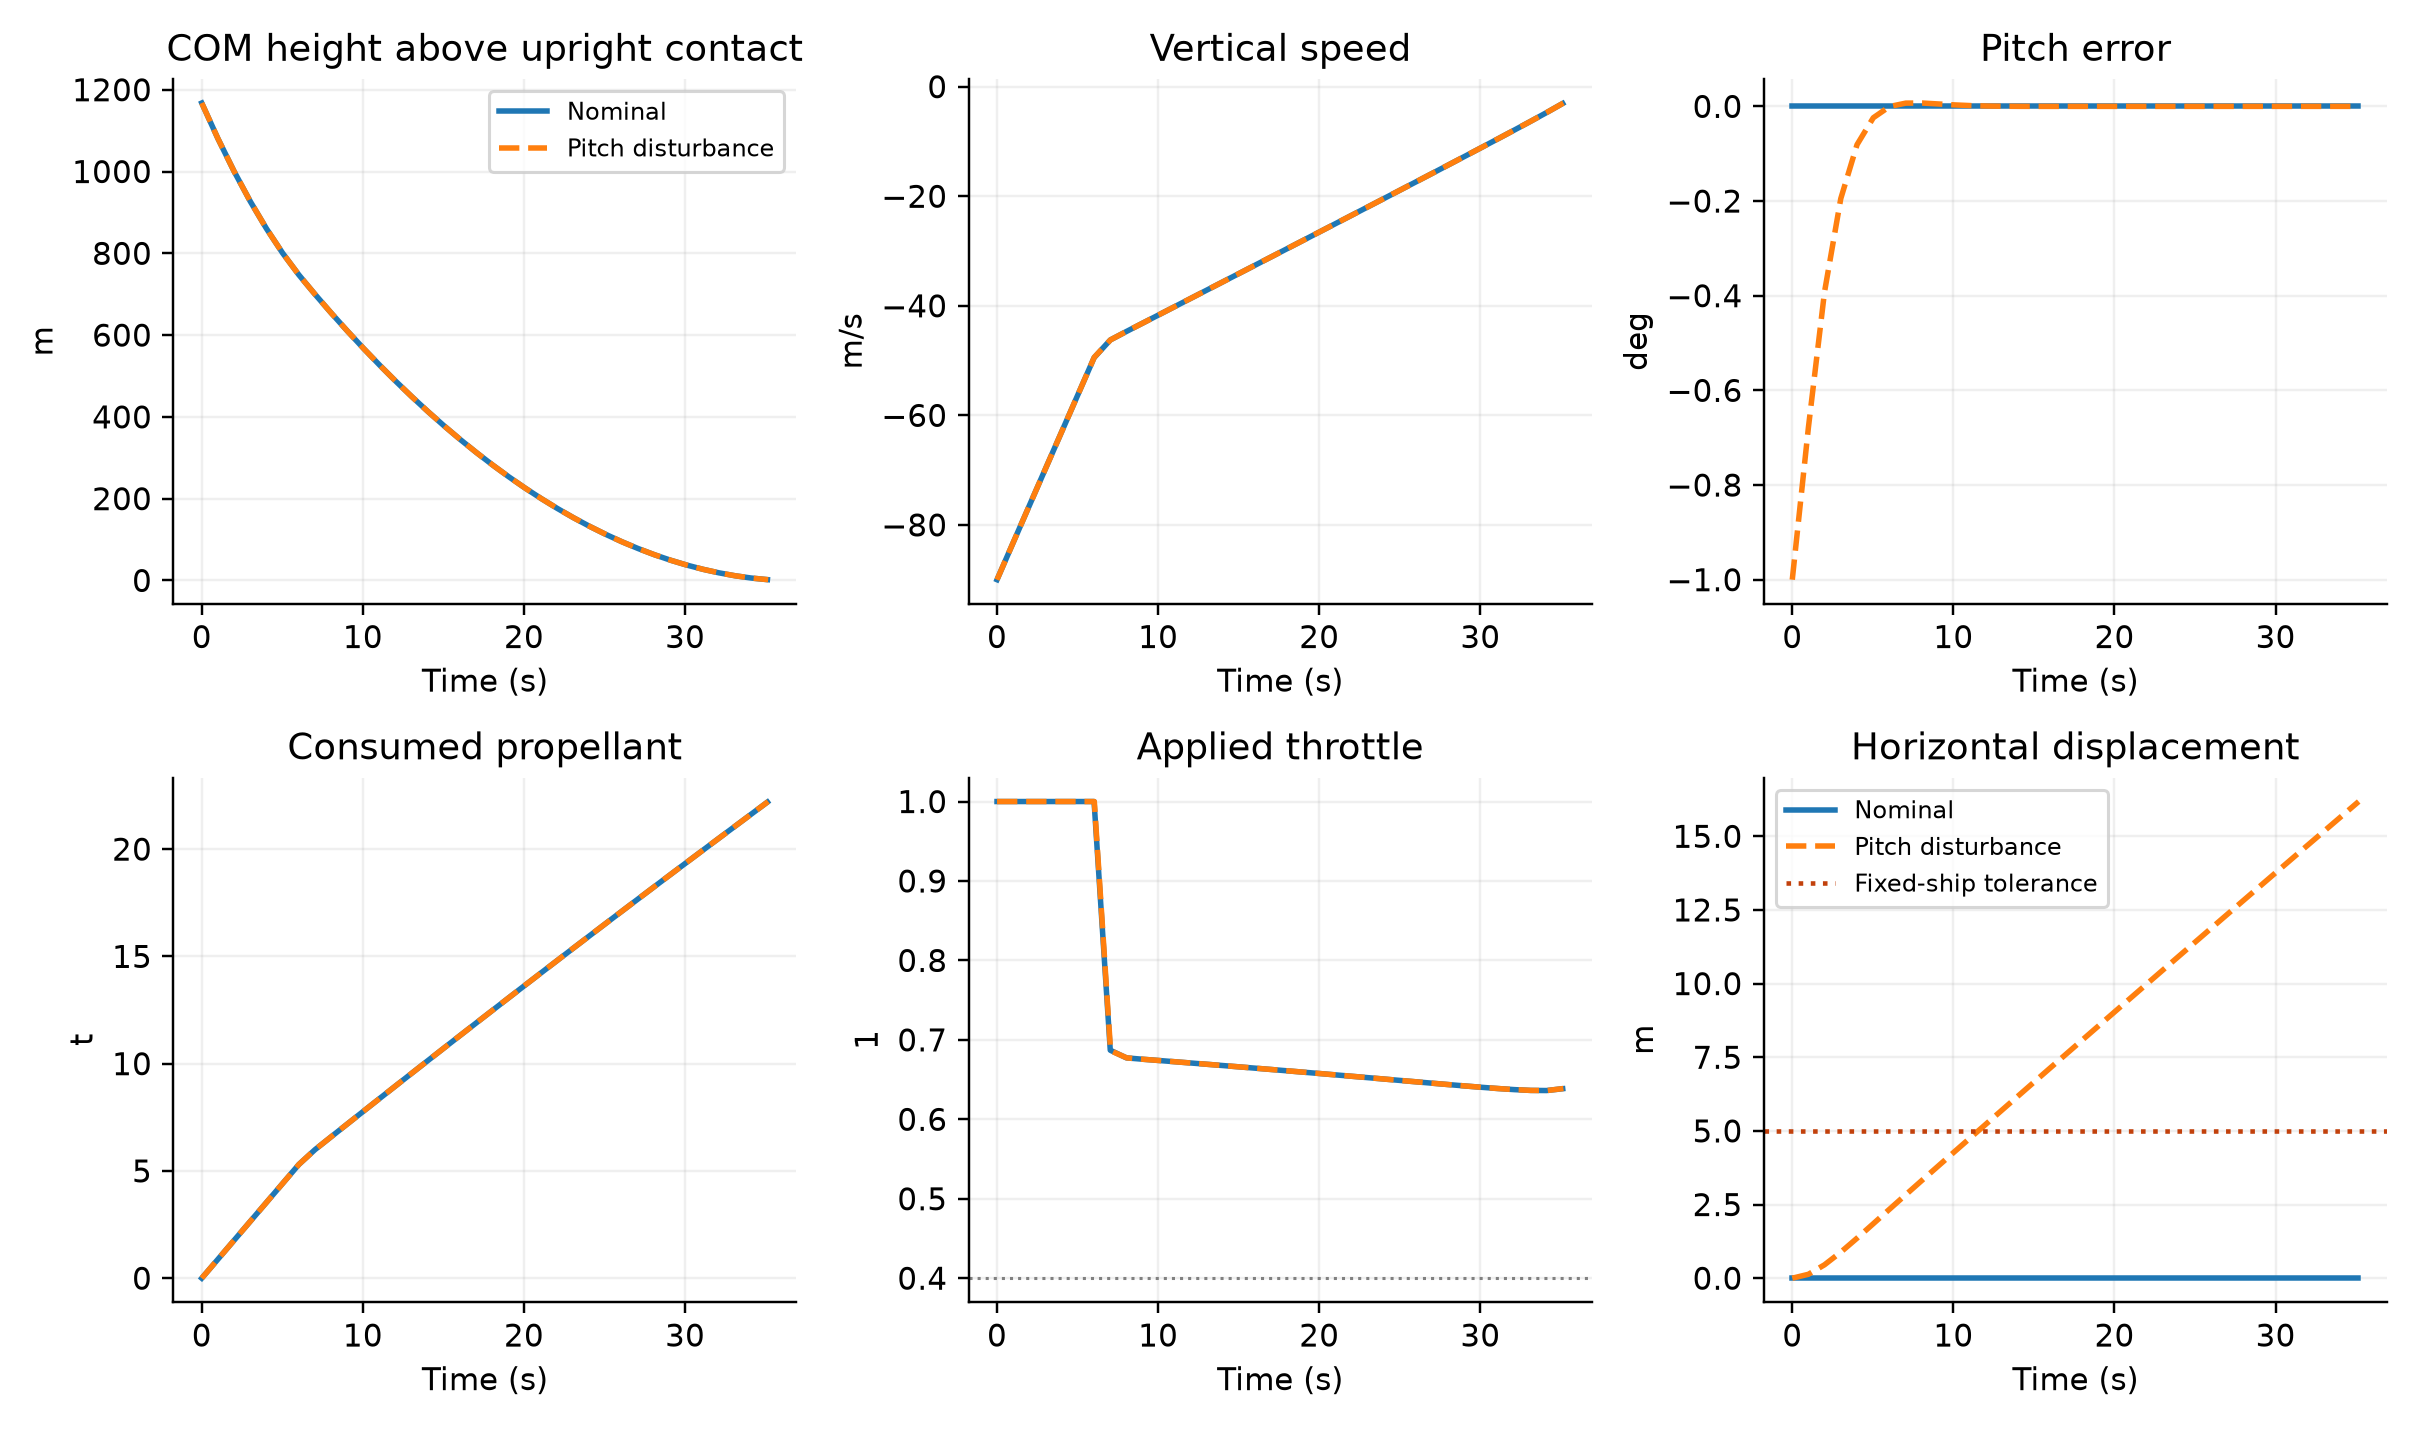
\includegraphics[width=\linewidth]{figure/p1-terminal.png}
\caption{Local powered-braking verification, not a separation-to-landing solution. The disturbed case starts at $89^\circ$ pitch with 0.005 rad/s pitch rate. The 5 m line highlights that position capture is not guaranteed by attitude recovery.}\label{fig:terminal}
\end{figure}

\clearpage
\section{Internal Verification}
\subsection{P1 Internal Verification and Numerical Convergence}
The verification suite tests implementation consistency and known limiting solutions; no flight-data validation is claimed. Standard-atmosphere base pressures at 0, 11, 20, 32, and 47 km geopotential altitude agree with rounded reference values within $4.8\times10^{-6}$ relative error. Out-of-range atmospheric queries are rejected. A vertical vacuum coast conserves the modeled specific mechanical energy to $7.5\times10^{-9}$ J/kg over 20 s. Constant-thrust mass history and horizontal ideal-rocket velocity agree with their analytic expressions to $7.6\times10^{-10}$ kg and $2.9\times10^{-14}$ m/s, respectively, in the chosen tests. These small residuals apply to those tests and do not measure real-world accuracy.

Pure axial and pure crossflow force limits, static pressure-center torque, torque-free rotation, damping sign, gimbal sign, and air-relative dissipativity are checked. For pure centered rotation, Eq.~\eqref{eq:rotation} provides an independent integral. Midpoint-strip relative errors are 2\%, 0.5\%, 0.125\%, 0.03125\%, and 0.0078125\% for 10, 20, 40, 80, and 160 strips. Thus the default 20-strip rotational torque has a 0.5\% quadrature error in this limiting case; this is distinct from uncertainty in the aerodynamic coefficients.

A four-second smooth unpowered trajectory is compared with a 0.00125 s reference using the same equations. Position differences decrease from $9.75\times10^{-7}$ m at 0.08 s to $2.76\times10^{-10}$ m at 0.01 s. Since force laws contain absolute values and feedback contains clipping, fourth-order behavior is not assumed across every nonsmooth transition. Figure~\ref{fig:convergence} separates smooth integration, strip quadrature, and touchdown-event checks.
\begin{table}[htbp]\centering
\caption{Local terminal-event convergence. All rows satisfy the selected speed, attitude, and reserve criteria; this table does not test fixed-ship position capture.}
\begin{tabular}{rrrr}\toprule
Step (s)&Contact time (s)&$v_h$ (m/s)&Consumed (kg)\\\midrule
0.080&35.975945&-1.502940&22679.544\\
0.040&35.975286&-1.503756&22679.191\\
0.020&35.975097&-1.502978&22679.139\\
0.010&35.975063&-1.502986&22679.123\\
0.005&35.975047&-1.502909&22679.119\\\bottomrule
\end{tabular}
\end{table}
Between the final two steps, consumption changes by 0.00384 kg and contact time by $1.60\times10^{-5}$ s. Event speed differences are not monotonic, so no fourth-order contact-convergence claim is made. The fuel-depletion guard is verified to avoid dry-mass overshoot, while exact depletion-time localization remains outside this conservative guard's contract.
\begin{figure}[htbp]\centering
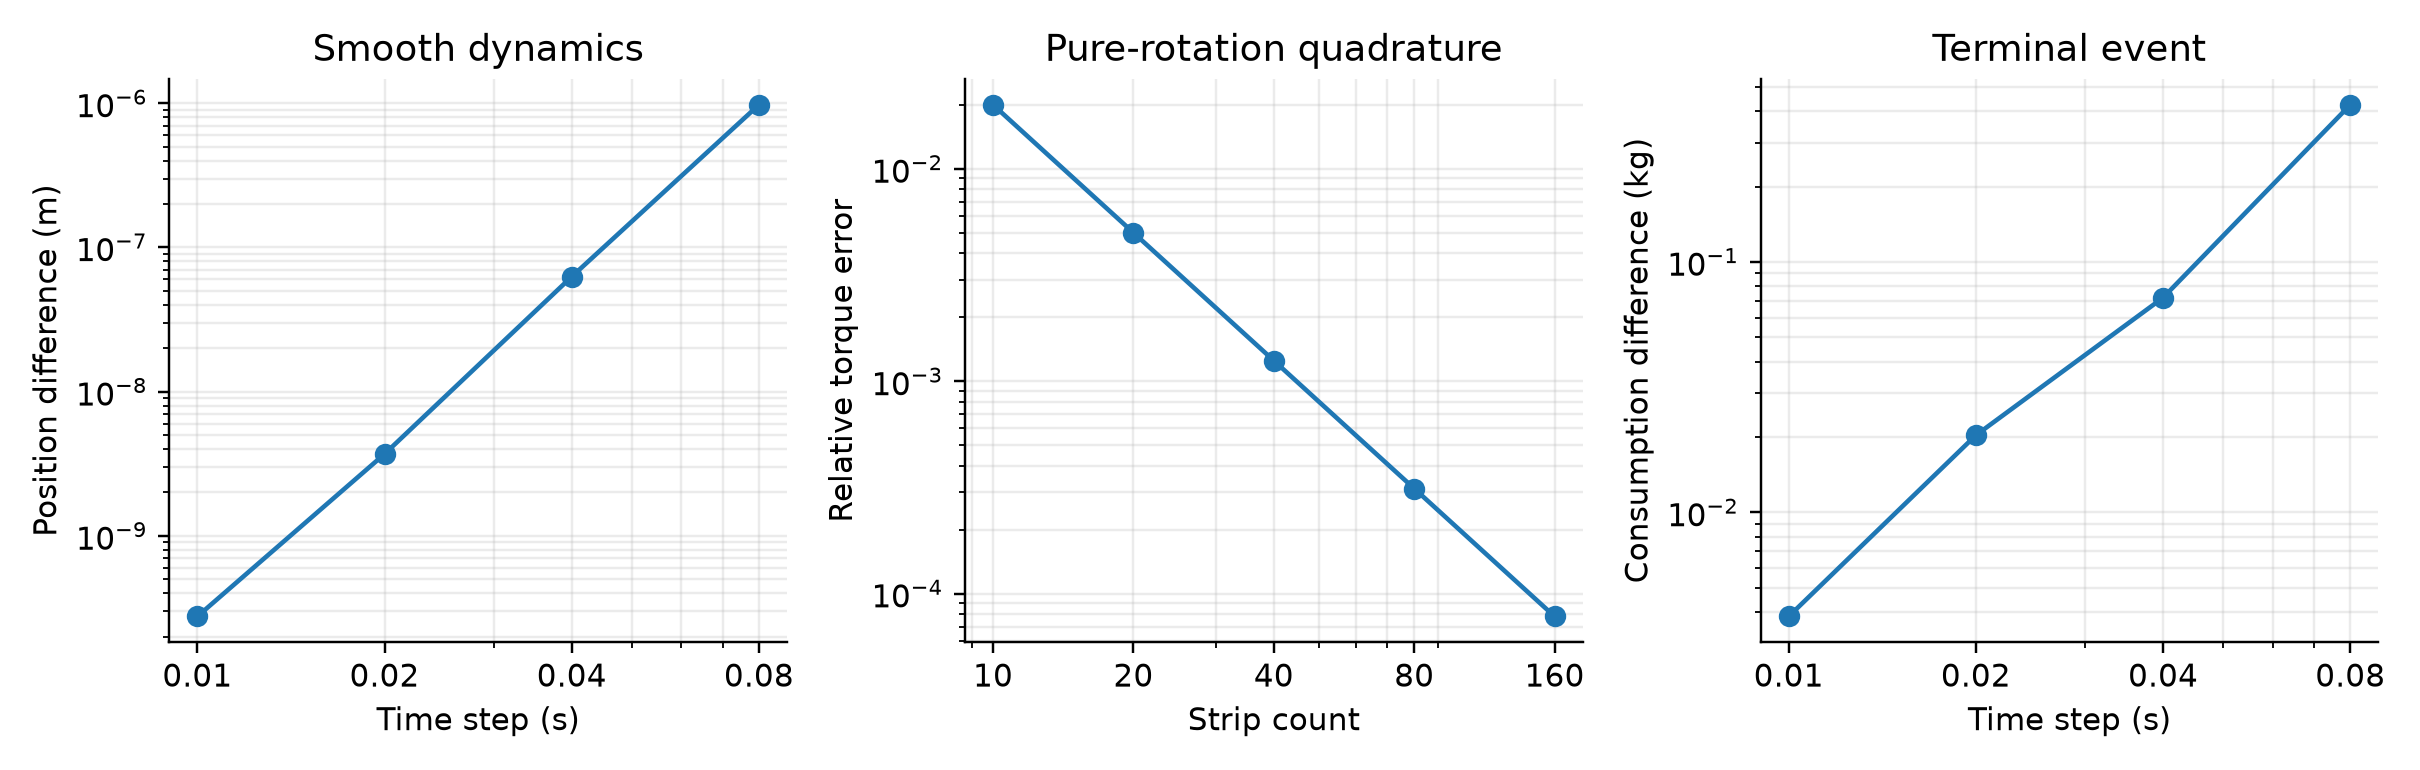
\includegraphics[width=\linewidth]{figure/p1-convergence.png}
\caption{Independent numerical error sources. Left: smooth-trajectory position difference relative to a finer same-model integration. Middle: strip torque error against the analytic integral. Right: contact-consumption difference relative to the 0.005 s run.}\label{fig:convergence}
\end{figure}
The reference implementation and P1 checks are reproducible with \texttt{node src/verify-p1.mjs}. The remaining limitations are model-form uncertainty, actuator idealization, atmosphere range, local-plane/rotation approximations, and absent structural/thermal allowables. Whole-flight feasibility and fuel optimization are delegated to the next stage.

\clearpage
\begin{thebibliography}{9}
\bibitem{be4} Blue Origin. BE-4. Manufacturer webpage, accessed November 7, 2026. \url{https://www.blueorigin.com/es-MX/engines/be-4}.
\bibitem{cylinder} F. E. Gowen and E. W. Perkins. Drag of Circular Cylinders for a Wide Range of Reynolds Numbers and Mach Numbers. NACA-TN-2960, 1953.
\bibitem{atmosphere} NOAA, NASA, and USAF. U.S. Standard Atmosphere, 1976. NASA-TM-X-74335, 1976.
\bibitem{methaneStudy} Mars Sample Return Mission Utilizing In-Situ Propellant Production. NASA NTRS record 19950021840. Methane/oxygen performance discussion, Fig. 2.
\bibitem{problem} UPC 2026, Problem A: Landing a First-Stage Rocket Booster. User-provided problem image.
\end{thebibliography}
\end{document}
